\documentclass{article}

\usepackage{csquotes}
% 使用中文CJK包
\usepackage{CJK}
% 图像插入宏包
\usepackage{graphicx}
% 自定义颜色支持
\usepackage[usenames,dvipsnames]{color}
% 长表格跨页支持
\usepackage{longtable}
% 代码高亮支持
\usepackage{listings}
% 算法伪代码包
\usepackage[ruled,vlined]{algorithm2e}
% 自定义标题格式
\usepackage{titlesec}
% 扩展tabular样式
\usepackage{array}
% 添加页眉页脚
\usepackage{fancyhdr}
% 虚拟正文测试
\usepackage{lipsum}
% 数学环境包
\usepackage{amsmath}
% 首行缩进
\usepackage{indentfirst}
% 树状结构图
\usepackage{tree-dvips}
% 脚注环境
\usepackage{footnote}
% 定制表格线
\usepackage{makecell}
% tikz绘图包
\usepackage{tikz}
% URL超链接
\usepackage[dvips, colorlinks, linkcolor=black]{hyperref}
% 断行URL超链接
\usepackage{breakurl}


% hyperref中文兼容
\pdfstringdefDisableCommands{
\let\CJK@XX\relax
\let\CJK@XXX\relax
\let\CJK@XXXp\relax
\let\CJK@XXXX\relax
\let\CJK@XXXXp\relax
}

\usetikzlibrary{positioning,shapes,shadows,arrows}


% 设置脚注在table中可用
\makesavenoteenv{table}

% 设置标题格式
%\titleformat{\chapter}{\raggedright\Huge\bfseries}{Chapter \thechapter}{1em}{}

% 设置默认字体族, 具体字体请查看texdoc psnfss2e

% 设置Roman字体为Palatino
\renewcommand{\rmdefault}{ppl} 
% 设置TypeWriter字体为Courier
\renewcommand{\ttdefault}{pcr} 

% 设置行距
\setlength{\parskip}{1ex}

% 定义需要的颜色

\definecolor{lightgray}{RGB}{230,230,230}
\definecolor{lightblue}{RGB}{224, 224, 255}
\definecolor{darkblue}{RGB}{192, 192, 255}
\definecolor{lightpink}{RGB}{255, 224, 224}
\definecolor{darkpink}{RGB}{255, 192, 192}
\definecolor{keywordyellow}{RGB}{255, 204, 0}
\definecolor{keywordred}{RGB}{194, 58, 0}
\definecolor{numbercolor}{RGB}{102, 51, 0}

% 设置代码风格

% 定义C语言代码风格
\lstdefinestyle{ccode}
{ 
    language=C, 
    numbers=left, 
    numberstyle=\color{numbercolor},
    basicstyle=\scriptsize\ttfamily\bfseries,
    keywordstyle=\color{blue}, 
    commentstyle=\color{PineGreen},
    stringstyle=\color{red}, 
    frame=shadowbox, 
    frameround=tttt,
    breaklines=true,
    backgroundcolor=\color{lightgray} }

% 定义汇编语言代码风格
\lstdefinestyle{acode}
{ 
    language=,
    morekeywords=[1]{mov, movl, movb, movw, orl, xorw, cli, cld, inb, testb, test, jnz, push, pop, jmp, call, lea, add, sub, ret, jle, outb, ljmp, lgdt, cmp, jne, popal, int, jns, pushw, pushal, pushl, popfl, addl, subl},
    morekeywords=[2]{ax, bx, cx, dx, eax, ebx, ecx, edx, cr0, cr1, cr2, cr3, al, ds, es, ss, esp, ebp, esi, edi}, 
    morekeywords=[3]{data, text, bss},
    morekeywords=[4]{long, align, p2align, ascii, fill, globl, space, set, rept, byte, word},
    morecomment=[l]\#,
    numbers=left, 
    numberstyle=\color{numbercolor},
    basicstyle=\scriptsize\ttfamily\bfseries,
    keywordstyle=[1]\color{blue}, 
    keywordstyle=[2]\color{keywordyellow},
    keywordstyle=[3]\color{orange},
    keywordstyle=[4]\color{keywordred},
    commentstyle=\color{PineGreen},
    stringstyle=\color{red}, 
    frame=shadowbox, 
    frameround=tttt,
    breaklines=true,
    backgroundcolor=\color{lightgray} }

    
% 定义命令行输出风格
\lstdefinestyle{console}
{
    language=bash, 
    numbers=none, 
    frame=tRBl,
    basicstyle=\scriptsize\color{green}\ttfamily\bfseries,     
    backgroundcolor=\color{black}}


% 定义exercise输出风格
\lstdefinestyle{exercise}
{
    numbers=none, 
    frame=tRBl,
    breaklines=true,
    breakindent=0pt,
    framexleftmargin=1em,
    framexrightmargin=1em,
    framextopmargin=2ex,
    framexbottommargin=2ex,
    xleftmargin=0.05\linewidth,
    xrightmargin=0.05\linewidth,
    basicstyle=\scriptsize\ttfamily\mdseries,   
    moredelim=[is][\ttfamily\bfseries]{|}{|},
    framerule=0.8pt,
    rulecolor=\color{darkblue}, 
    backgroundcolor=\color{lightblue}}
    

% 定义challenge输出风格
\lstdefinestyle{challenge}
{
    numbers=none, 
    frame=tRBl,
    breaklines=true,
    breakindent=0pt,
    framexleftmargin=1em,
    framexrightmargin=1em,
    framextopmargin=2ex,
    framexbottommargin=2ex,
    xleftmargin=0.05\linewidth,
    xrightmargin=0.05\linewidth,
    basicstyle=\scriptsize\ttfamily\mdseries,   
    moredelim=[is][\ttfamily\bfseries]{|}{|},
    framerule=0.8pt,
    rulecolor=\color{darkpink}, 
    backgroundcolor=\color{lightpink}}
    


% 非常重要, listings关闭非ASCII字符兼容
\lstset{extendedchars=false}


% 定义问题的答案格式
\newcommand{\highlight}[1]{{\bfseries \color{red}  #1}}
% 定义函数名格式
\newcommand{\funcname}[1]{{\ttfamily \small #1}}




\pagestyle{fancy}
\begin{document}
\begin{CJK*}{UTF8}{gkai}

\lhead{操作系统实习报告}
\rhead{张弛, 00848231}
\title{操作系统JOS实习第四次报告}
\author{张弛 \hspace{1ex} 00848231, \\
        zhangchitc@gmail.com}

\maketitle
% 记得在文档末尾插入\clearpage
\tableofcontents
\newpage

\section{Introduction}

我在实验中主要参考了华中科技大学邵志远老师写的JOS实习指导,在邵老师的主页上\burl{http://grid.hust.edu.cn/zyshao/OSEngineering.htm} 可以找到。但是这次实验的指导远远不如lab1的指导详尽,所以我这里需要补充的内容会很多。

内联汇编请参考邵老师的第二章讲义,对于语法讲解的很详细。


\section{User-level Environment Creation and Cooperative Multitasking}

这个部分的MIT文档讲解的比较详细,细节的串接都比较清楚。结合代码的注释写起来不是很困难。

\subsection{Round-Robin Scheduling}

\begin{lstlisting}[style=exercise]
|Exercise 1.| Implement round-robin scheduling in sched_yield() as described above. Don't forget to modify syscall() to dispatch sys_yield().

Modify kern/init.c to create three (or more!) environments that all run the program user/yield.c. You should see the environments switch back and forth between each other five times before terminating, like this:

...
Hello, I am environment 00001001.
Hello, I am environment 00001002.
Hello, I am environment 00001003.
Back in environment 00001001, iteration 0.
Back in environment 00001002, iteration 0.
Back in environment 00001003, iteration 0.
Back in environment 00001001, iteration 1.
Back in environment 00001002, iteration 1.
Back in environment 00001003, iteration 1.
...
After the yield programs exit, the idle environment should run and invoke the JOS kernel debugger. If any of this does not happen, then fix your code before proceeding.
\end{lstlisting}

\funcname{sched\_yield()} 函数比较简单,直接贴代码了:

\begin{lstlisting}[style=ccode, title={\scriptsize \ttfamily \bfseries kern/sched.c: sched\_yield()}]
void
sched_yield(void)
{
    struct Env *curenvptr = curenv;

    if (curenv == NULL)
        curenvptr = envs;

    int round = 0;
    for (curenvptr ++; round < NENV; round ++, curenvptr ++) {

        if (curenvptr >= envs + NENV) {
            curenvptr = envs + 1;
        }

        if (curenvptr->env_status == ENV_RUNNABLE)
            env_run (curenvptr);
    }

    // Run the special idle environment when nothing else is runnable.
    if (envs[0].env_status == ENV_RUNNABLE)
        env_run(&envs[0]);
    else {
        cprintf("Destroyed all environments - nothing more to do!\n");
        while (1)
            monitor(NULL);
	}
}
\end{lstlisting}

然后修改kern/syscall.c添加相关的分发机制,然后在kern/init.c中系统启动之初创建user\_idle以后再创建user\_yield,这个用户程序的功能就是作五次\funcname{sys\_yield()}的系统调用,并且切换时打印相关的消息:

\begin{lstlisting}[style=ccode, title={\scriptsize \ttfamily \bfseries kern/init.c: i386\_init()}]
	// Should always have an idle process as first one.
	ENV_CREATE(user_idle);
        ENV_CREATE(user_yield);
        ENV_CREATE(user_yield);
        ENV_CREATE(user_yield);
\end{lstlisting}

那么启动JOS后应该打印出下列消息:(注意,因为是使用Round Robin策略切换,所以顺序应该是确定的)


\begin{lstlisting}[style=console]
qemu -hda obj/kern/kernel.img -serial mon:stdio
6828 decimal is 15254 octal!
Hooray! Passed all test cases for stdlib!!
Physical memory: 66556K available, base = 640K, extended = 65532K
check_page_alloc() succeeded!
page_check() succeeded!
check_boot_pgdir() succeeded!
enabled interrupts: 1 2
	     Setup timer interrupts via 8259A
enabled interrupts: 0 1 2
	     unmasked timer interrupt
[00000000] new env 00001000
[00000000] new env 00001001
[00000000] new env 00001002
[00000000] new env 00001003
Hello, I am environment 00001001.
Hello, I am environment 00001002.
Hello, I am environment 00001003.
Back in environment 00001001, iteration 0.
Back in environment 00001002, iteration 0.
Back in environment 00001003, iteration 0.
Back in environment 00001001, iteration 1.
Back in environment 00001002, iteration 1.
Back in environment 00001003, iteration 1.
Back in environment 00001001, iteration 2.
Back in environment 00001002, iteration 2.
Back in environment 00001003, iteration 2.
Back in environment 00001001, iteration 3.
Back in environment 00001002, iteration 3.
Back in environment 00001003, iteration 3.
Back in environment 00001001, iteration 4.
All done in environment 00001001.
[00001001] exiting gracefully
[00001001] free env 00001001
Back in environment 00001002, iteration 4.
All done in environment 00001002.
[00001002] exiting gracefully
[00001002] free env 00001002
Back in environment 00001003, iteration 4.
All done in environment 00001003.
[00001003] exiting gracefully
[00001003] free env 00001003
Welcome to the JOS kernel monitor!
Type 'help' for a list of commands.
\end{lstlisting}

\vspace{2em}
\hrule
\vspace{2em}


\begin{lstlisting}[style=exercise]
|Question|

In your implementation of env_run() you should have called lcr3(). Before and after the call to lcr3(), your code makes references (at least it should) to the variable e, the argument to env_run. Upon loading the %cr3 register, the addressing context used by the MMU is instantly changed. But a virtual address (namely e) has meaning relative to a given address context--the address context specifies the physical address to which the virtual address maps. Why can the pointer e be dereferenced both before and after the addressing switch?
\end{lstlisting}

我们先来回顾一下\funcname{env\_run()}里的具体代码:


\begin{lstlisting}[style=ccode, title={\scriptsize \ttfamily \bfseries kern/env.c: env\_run()}]
void
env_run(struct Env *e)
{
    if (curenv != e) {
        curenv = e;
        curenv->env_runs ++;
        lcr3 (curenv->env_cr3);
    }

    env_pop_tf (&curenv->env_tf);

    panic("env_run not yet implemented");
}
\end{lstlisting}

我们尝试在未切换到用户页地址之前打印出e在系统页表中的地址,看看是个什么样子:

\begin{lstlisting}[style=console]
[00000000] new env 00001000
[00000000] new env 00001001
[00000000] new env 00001002
[00000000] new env 00001003
zhangchi: e ptr = f01f207c, KERNBASE = f0000000
zhangchi: e ptr = f01f207c, KERNBASE = f0000000
Hello, I am environment 00001001.
zhangchi: e ptr = f01f207c, KERNBASE = f0000000
zhangchi: e ptr = f01f20f8, KERNBASE = f0000000
zhangchi: e ptr = f01f20f8, KERNBASE = f0000000
Hello, I am environment 00001002.
\end{lstlisting}

可以看到e的地址是在KERNBASE以上的系统区,而很明显,在所有用户页地址空间里,KERNBASE以上的空间都是和boot\_pgdir是一样的,指向同一片物理内存区域。所以我们在切换页表的前后e是不受影响的。

\subsection{System Calls for Environment Creation}

这个小节里我一开始最迷惑的就是这个\funcname{sys\_exofork()}对于父进程和子进程的返回值的区别。因为操作系统应该是可以递归的让子进程不断创建子进程的,\highlight{那这里子进程调用返回0又是如何解释?如果他调用老是返回0那如何让其递归的创建子进程?}

这里需要重申一下\funcname{fork()}的机制,因为创建出的子进程和父亲是同一进程,即它们在汇编代码级别是一模一样的,父亲创建一个子进程应该是在一个int 30的中断调用里完成的,这个中断去调用相应的系统\funcname{fork()}代码。比如我们可以看看obj/user/dumbfork.asm看看相关的代码:

\begin{lstlisting}[style=acode, firstnumber=118, title={\scriptsize \ttfamily \bfseries obj/user/dumbfork.asm}]
envid_t
dumbfork(void)
{
  800119:	55                   	push   %ebp
  80011a:	89 e5                	mov    %esp,%ebp
  80011c:	53                   	push   %ebx
  80011d:	83 ec 24             	sub    $0x24,%esp
static __inline envid_t sys_exofork(void) __attribute__((always_inline));
static __inline envid_t
sys_exofork(void)
{
	envid_t ret;
	__asm __volatile("int %2"
  800120:	bb 07 00 00 00       	mov    $0x7,%ebx
  800125:	89 d8                	mov    %ebx,%eax
  800127:	cd 30                	int    $0x30
  800129:	89 c3                	mov    %eax,%ebx
	// The kernel will initialize it with a copy of our register state,
	// so that the child will appear to have called sys_exofork() too -
	// except that in the child, this "fake" call to sys_exofork()
	// will return 0 instead of the envid of the child.
	envid = sys_exofork();
	if (envid < 0)
  80012b:	85 c0                	test   %eax,%eax
  80012d:	79 20                	jns    80014f <dumbfork+0x36>
		panic("sys_exofork: %e", envid);
\end{lstlisting}

这个时候,中断调用后创建的子进程和父进程有一样的进程状态,父亲的调用完以后因为这个\funcname{fork()}有一个返回值代表子进程的pid,这个返回值按照lab3的规定应该是在eax里的,所以int 30的下一句汇编代码应该就是把这个eax赋值给相应的变量,如上面代码中800129地址的指令。但是如果切换到子进程继续运行的话,\highlight{不能让它也接受一个和父进程一样的eax(因为这个时候eax不就是它自己的pid么)},所以为了区分就让它的返回值等于0就好了。即让其eax寄存器设置为0.

其他就没什么太大的疑问了。

\vspace{2em}

\begin{lstlisting}[style=exercise]
|Exercise 2.| Implement the system calls described above in kern/syscall.c. You will need to use various functions in kern/pmap.c and kern/env.c, particularly envid2env(). For now, whenever you call envid2env(), pass 1 in the checkperm parameter. Be sure you check for any invalid system call arguments, returning -E_INVAL in that case. Test your JOS kernel with user/dumbfork and make sure it works before proceeding.
\end{lstlisting}

我们一个函数一个函数的看,首先是刚才提到的\funcname{sys\_exofork()}

\begin{lstlisting}[style=ccode, title={\scriptsize \ttfamily \bfseries kern/syscall.c: sys\_exofork()}]
static envid_t
sys_exofork(void)
{
    struct Env *newenv;
    int r;

    if ((r = env_alloc (&newenv, sys_getenvid())) < 0) 
        return r;

    // set not runnnable
    newenv->env_status = ENV_NOT_RUNNABLE;

    // copy trapframe 
    newenv->env_tf = curenv->env_tf;

    // make the child env's return value zero
    newenv->env_tf.tf_regs.reg_eax = 0;

    return newenv->env_id;
}
\end{lstlisting}

这里最重要的就是第17行,让创建好的子进程的eax为0,那么它从系统调用得到的返回值就是0了。

然后是\funcname{env\_set\_status()},很简单,照着注释写就行

\begin{lstlisting}[style=ccode, title={\scriptsize \ttfamily \bfseries kern/syscall.c: env\_set\_status()}]
static int
sys_env_set_status(envid_t envid, int status)
{
    if (status != ENV_RUNNABLE && status != ENV_NOT_RUNNABLE)
        return -E_INVAL;

    struct Env *envptr;
    int r;

    if ((r = envid2env (envid, &envptr, 1)) < 0)
        return r;

    envptr->env_status = status;

    return 0;
}
\end{lstlisting}

接下来是\funcname{env\_page\_alloc()}

\begin{lstlisting}[style=ccode, title={\scriptsize \ttfamily \bfseries kern/syscall.c: sys\_page\_alloc()}]
static int
sys_page_alloc(envid_t envid, void *va, int perm)
{
    if (va >= (void *)UTOP)
        return -E_INVAL;

    if ((perm & PTE_U) == 0 || (perm & PTE_P) == 0)
        return -E_INVAL;
    // PTE_USER = PTE_U | PTE_P | PTE_W | PTE_AVAIL
    if ((perm & ~PTE_USER) > 0)
        return -E_INVAL;

    struct Env *e;
    if (envid2env (envid, &e, 1) < 0)
        return -E_BAD_ENV;

    struct Page *p;
    if (page_alloc (&p) < 0)
        return -E_NO_MEM;

    if (page_insert (e->env_pgdir, p, va, perm) < 0) {
        page_free (p);
        return -E_NO_MEM;
    }

    memset (page2kva (p), 0, PGSIZE);

    return 0;
}
\end{lstlisting}

注意,这里最重要的是最后一句memset,这个在注释中没有提及,但是在邵老师的讲义里面提到了,\highlight{申请了新页面以后注意要给用户进程清空以防止脏数据的情况}。请认真阅读绍老师的讲义。

然后来看\funcname{sys\_page\_map()}

\begin{lstlisting}[style=ccode, title={\scriptsize \ttfamily \bfseries kern/syscall.c: sys\_page\_map()}]
static int
sys_page_map(envid_t srcenvid, void *srcva,
	     envid_t dstenvid, void *dstva, int perm)
{
    if (srcva >= (void *)UTOP || ROUNDUP (srcva, PGSIZE) != srcva
    ||  dstva >= (void *)UTOP || ROUNDUP (dstva, PGSIZE) != dstva)
        return -E_INVAL;

    if ((perm & PTE_U) == 0 || (perm & PTE_P) == 0)
        return -E_INVAL;
    // PTE_USER = PTE_U | PTE_P | PTE_W | PTE_AVAIL
    if ((perm & ~PTE_USER) > 0)
        return -E_INVAL;

    struct Env *srcenv;
    if (envid2env (srcenvid, &srcenv, 1) < 0)
        return -E_BAD_ENV;

    struct Env *dstenv;
    if (envid2env (dstenvid, &dstenv, 1) < 0)
        return -E_BAD_ENV;

    pte_t *pte;
    struct Page *p = page_lookup (srcenv->env_pgdir, srcva, &pte);
    if (p == NULL || ((perm & PTE_W) > 0 && (*pte & PTE_W) == 0))
        return -E_INVAL;

    if (page_insert (dstenv->env_pgdir, p, dstva, perm) < 0)
        return -E_NO_MEM;

    return 0;
}
\end{lstlisting}

没什么需要注意的地方,继续看\funcname{sys\_page\_unmap()}


\begin{lstlisting}[style=ccode, title={\scriptsize \ttfamily \bfseries kern/syscall.c: sys\_page\_unmap()}]
static int
sys_page_unmap(envid_t envid, void *va)
{
    if (va >= (void *)UTOP || ROUNDUP (va, PGSIZE) != va)
        return -E_INVAL;

    struct Env *env;
    if (envid2env (envid, &env, 1) < 0)
        return -E_BAD_ENV;

    page_remove (env->env_pgdir, va);

    return 0;
}
\end{lstlisting}

到此为止这个Exercise涉及的全部代码就已经完成了,当然还有我们要对相应的系统调用号添加分发逻辑。然后我们来考虑运行一下user/dumbfork,首先来看看它的代码,这里节选它的主函数段:


\begin{lstlisting}[style=ccode, firstnumber=9, title={\scriptsize \ttfamily \bfseries user/dumbfork.c: umain()}]
void
umain(void)
{
	envid_t who;
	int i;

	// fork a child process
	who = dumbfork();

	// print a message and yield to the other a few times
	for (i = 0; i < (who ? 10 : 20); i++) {
		cprintf("%d: I am the %s!\n", i, who ? "parent" : "child");
		sys_yield();
	}
}
\end{lstlisting}

这个代码的逻辑就是:父进程创建一个子进程,然后每次打印一条信息以后交出控制权,并且让父进程重复10次而子进程重复20次。

这个逻辑已经很明显了,我们尝试这运行一下,输入make run-dumbfork:


\begin{lstlisting}[style=console]
qemu -hda obj/kern/kernel.img -serial mon:stdio
6828 decimal is 15254 octal!
Hooray! Passed all test cases for stdlib!!
Physical memory: 66556K available, base = 640K, extended = 65532K
check_page_alloc() succeeded!
page_check() succeeded!
check_boot_pgdir() succeeded!
enabled interrupts: 1 2
	     Setup timer interrupts via 8259A
enabled interrupts: 0 1 2
	     unmasked timer interrupt
[00000000] new env 00001000
[00000000] new env 00001001
[00001001] new env 00001002
0: I am the parent!
0: I am the child!
1: I am the parent!
1: I am the child!
2: I am the parent!
2: I am the child!
3: I am the parent!
3: I am the child!
4: I am the parent!
4: I am the child!
5: I am the parent!
5: I am the child!
6: I am the parent!
6: I am the child!
7: I am the parent!
7: I am the child!
8: I am the parent!
8: I am the child!
9: I am the parent!
9: I am the child!
[00001001] exiting gracefully
[00001001] free env 00001001
10: I am the child!
11: I am the child!
12: I am the child!
13: I am the child!
14: I am the child!
15: I am the child!
16: I am the child!
17: I am the child!
18: I am the child!
19: I am the child!
[00001002] exiting gracefully
[00001002] free env 00001002
Welcome to the JOS kernel monitor!
Type 'help' for a list of commands.
\end{lstlisting}

和程序的预期逻辑是一致的。


\section{Copy-on-Write Fork}

\subsection{User-level page fault handling}

\subsection{Setting the Page Fault Handler}

\begin{lstlisting}[style=exercise]
|Exercise 3.| Implement the sys_env_set_pgfault_upcall system call. Be sure to enable permission checking when looking up the environment ID of the target environment, since this is a "dangerous" system call.
\end{lstlisting}

很简单:

\begin{lstlisting}[style=ccode, title={\scriptsize \ttfamily \bfseries kern/syscall.c: sys\_env\_set\_pgfault\_upcall()}]
static int
sys_env_set_pgfault_upcall(envid_t envid, void *func)
{
    struct Env *e;
    if (envid2env (envid, &e, 1) < 0)
        return -E_BAD_ENV;

    e->env_pgfault_upcall = func;

    return 0;
}
\end{lstlisting}


\subsection{Normal and Exception Stacks in User Environments}

首先梳理一下几个栈之间的关系。根据inc/memlayout.h中对于虚拟地址空间的描述,他们的布局如下:

\begin{lstlisting}[style=ccode, title={\scriptsize \ttfamily \bfseries inc/memlayout.h}]
/*
 * Virtual memory map:                                Permissions
 *                                                    kernel/user
 *
 *    4 Gig -------->  +------------------------------+
 *                     |                              | RW/--
 *                     ~~~~~~~~~~~~~~~~~~~~~~~~~~~~~~~~
 *                     :              .               :
 *                     :              .               :
 *                     :              .               :
 *                     |~~~~~~~~~~~~~~~~~~~~~~~~~~~~~~| RW/--
 *                     |                              | RW/--
 *                     |   Remapped Physical Memory   | RW/--
 *                     |                              | RW/--
 *    KERNBASE ----->  +------------------------------+ 0xf0000000
 *                     |  Cur. Page Table (Kern. RW)  | RW/--  PTSIZE
 *    VPT,KSTACKTOP--> +------------------------------+ 0xefc00000      --+
 *                     |         Kernel Stack         | RW/--  KSTKSIZE   |
 *                     | - - - - - - - - - - - - - - -|                 PTSIZE
 *                     |      Invalid Memory (*)      | --/--             |
 *    ULIM     ------> +------------------------------+ 0xef800000      --+
 *                     |  Cur. Page Table (User R-)   | R-/R-  PTSIZE
 *    UVPT      ---->  +------------------------------+ 0xef400000
 *                     |          RO PAGES            | R-/R-  PTSIZE
 *    UPAGES    ---->  +------------------------------+ 0xef000000
 *                     |           RO ENVS            | R-/R-  PTSIZE
 * UTOP,UENVS ------>  +------------------------------+ 0xeec00000
 * UXSTACKTOP -/       |     User Exception Stack     | RW/RW  PGSIZE
 *                     +------------------------------+ 0xeebff000
 *                     |       Empty Memory (*)       | --/--  PGSIZE
 *    USTACKTOP  --->  +------------------------------+ 0xeebfe000
 *                     |      Normal User Stack       | RW/RW  PGSIZE
 *                     +------------------------------+ 0xeebfd000
 *                     |                              |
 *                     |                              |
 *                     ~~~~~~~~~~~~~~~~~~~~~~~~~~~~~~~~
 *                     .                              .
 *                     .                              .
 *                     .                              .
 *                     |~~~~~~~~~~~~~~~~~~~~~~~~~~~~~~|
 *                     |     Program Data & Heap      |
 *    UTEXT -------->  +------------------------------+ 0x00800000
\end{lstlisting}

一共有三个栈:

\begin{description}
\item[$ [\mathrm{KSTACKTOP}, \mathrm{KSTACKTOP} - \mathrm{KSTKSIZE}) $] :\newline
内核态系统栈

\item[$ [\mathrm{UXSTACKTOP}, \mathrm{UXSTACKTOP} - \mathrm{PGSIZE}) $] :\newline
用户态错误处理栈

\item[$ [\mathrm{USTACKTOP}, \mathrm{UTEXT}) $] :\newline
用户态运行栈

\end{description}

他们之间的几个区别是:

\begin{itemize}
\item{\highlight{内核态系统栈}运行的是内核的相关程序,在这里我们关注的仅仅是\highlight{在有中断被触发以后},CPU会将自动将栈切换到内核栈上来。我们是在kern/trap.c的\funcname{idt\_init()}中进行相应设置的:

\begin{lstlisting}[style=ccode, title={\scriptsize \ttfamily \bfseries kern/trap.c: idt\_init()}]
	// Setup a TSS so that we get the right stack
	// when we trap to the kernel.
	ts.ts_esp0 = KSTACKTOP;
	ts.ts_ss0 = GD_KD;

	// Initialize the TSS field of the gdt.
	gdt[GD_TSS >> 3] = SEG16(STS_T32A, (uint32_t) (&ts),
					sizeof(struct Taskstate), 0);
	gdt[GD_TSS >> 3].sd_s = 0;

	// Load the TSS
	ltr(GD_TSS);

	// Load the IDT
	asm volatile("lidt idt_pd");
\end{lstlisting}

那么当一个中断被触发进入kern/trapentry.S中定义的中断服务程序时,所处在的栈就已经是内核栈了:

\begin{lstlisting}[style=acode, title={\scriptsize \ttfamily \bfseries kern/trapentry.S}]
/*
 * Lab 3: Your code here for _alltraps
 */
_alltraps:

    pushw    $0x0
    pushw    %ds
    pushw    $0x0
    pushw    %es
    pushal

    movl     $GD_KD, %eax
    
    movw     %ax, %ds
    movw     %ax, %es

    pushl    %esp

    call trap
\end{lstlisting}

这里push的指令全都是写入KSTACKTOP以下的空间的,为了形成一个Trapframe的内存结构,最后一个pushl \%esp是为了按照C Convention传入一个参数的句柄,因为trap 函数的定义为

\begin{lstlisting}[style=ccode, title={\scriptsize \ttfamily \bfseries kern/trap.c}]
void trap (struct Trapframe *tf) 
\end{lstlisting}

需要一个参数句柄。
}
\item{\highlight{用户运行栈}则是用户程序运行中使用的栈,初始是在创建用户进程初始时设置的,在kern/env.c的\funcname{env\_alloc()}中可以看到:

\begin{lstlisting}[style=ccode, title={\scriptsize \ttfamily \bfseries kern/env.c: env\_alloc()}]
	// Set up appropriate initial values for the segment registers.
	// GD_UD is the user data segment selector in the GDT, and 
	// GD_UT is the user text segment selector (see inc/memlayout.h).
	// The low 2 bits of each segment register contains the
	// Requestor Privilege Level (RPL); 3 means user mode.
	e->env_tf.tf_ds = GD_UD | 3;
	e->env_tf.tf_es = GD_UD | 3;
	e->env_tf.tf_ss = GD_UD | 3;
	e->env_tf.tf_esp = USTACKTOP;
	e->env_tf.tf_cs = GD_UT | 3;
	// You will set e->env_tf.tf_eip later.
\end{lstlisting}

这个时候其实其虚拟地址对应的地方只有一页的物理地址,在载入ELF文件时分配的:

\begin{lstlisting}[style=ccode, title={\scriptsize \ttfamily \bfseries kern/env.c: load\_icode()}]
    // LAB 3: Your code here.
    segment_alloc (e, (void*) (USTACKTOP - PGSIZE), PGSIZE);
\end{lstlisting}

如果用到了更多的空间,那么就会触发缺页中断,而转到内核栈上去运行中断处理程序。

注意用户运行栈是一边用一边分配的,而内核栈则固定了大小,而下面的用户态错误栈也是固定大小的。
}

\item{\highlight{用户态错误栈}是用户自己定义相应的中断处理程序后,相应处理程序运行时的栈。当用户进程调用前面的\funcname{sys\_env\_set\_pgfault\_upcall()}向系统注册缺页中断处理程序后,当用户程序触发缺页中断,那么
\begin{enumerate}
\item{首先系统陷入内核态,栈位置从\highlight{用户运行栈}切换到\highlight{内核栈},进入trap ()处理中断分发,进入page\_fault\_handler ()}
\item{当确认是用户程序而不是内核触发了缺页中断后,(内核的话就直接panic了),为其在用户错误栈里分配一个UTrapframe的大小(但是这时仍在\highlight{内核栈},我们只是在对应的页表空间里作的这样的操作)}
\item{把栈切换到\highlight{用户错误栈},运行相应的用户中断处理程序}
\item{最后返回用户程序,栈恢复到\highlight{用户运行栈}}
\end{enumerate}

那么这个栈是在哪里被指定的呢?\highlight{注意,只有注册了自己的缺页中断服务程序的用户进程才会分配用户错误栈},具体代码看到lib/pgfault.c中:

\begin{lstlisting}[style=ccode, title={\scriptsize \ttfamily \bfseries lib/pgfault.c: set\_pgfault\_handler()}]
void
set_pgfault_handler(void (*handler)(struct UTrapframe *utf))
{
	int r;

	if (_pgfault_handler == 0) {
		// First time through!
		// LAB 4: Your code here.
		panic("set_pgfault_handler not implemented");
	}

	// Save handler pointer for assembly to call.
	_pgfault_handler = handler;
}
\end{lstlisting}

在设置中断服务程序时,要作的工作之一就是为该进程的用户错误栈分配物理页面。只有这样,在进入内核的trap()中在错误栈里放置相应信息才不会触发缺页中断(细节在下节马上就会说到)

所以这个栈是自己创建的。
}
\end{itemize}

弄清楚这些栈的切换和设置关系对于我们下面要实现的系统调用非常重要。




\subsection{Invoking the User Page Fault Handler}


\begin{lstlisting}[style=exercise]
|Exercise 4.| Implement the code in page_fault_handler in kern/trap.c required to dispatch page faults to the user-mode handler. Be sure to take appropriate precautions when writing into the exception stack. (What happens if the user environment runs out of space on the exception stack?)
\end{lstlisting}

\funcname{page\_fault\_handler()} 在lab3中我们已经完成了对内核态触发的页错误的处理(如果在内核发生页错误,那么直接panic,以免发生更大的问题),这次的任务是完成在用户态中发生的页错误的处理。


有两种可能会造成缺页中断:

\begin{enumerate}
\item{用户程序正常运行中访问到一个错误地址,触发页错误中断}
\item{用户自己定义的页错误处理程序在运行时访问到错误地址,同样也会触发页错误中断}
\end{enumerate}

\highlight{注意!}有可能从第1种开始进入中断处理,然后2又触发2,又触发2 \ldots 造成中断处理的\highlight{递归}。


简单的来说,在\funcname{page\_fault\_handler()}要做的事情,就是将触发页错误的进程信息(可能是正常的用户程序,也可能是用户定义的页错误处理程序)以UTrapframe的形式压入用户的错误栈,然后进入用户的页错误处理程序开始运行。(用户的页错误处理程序会负责回到原来触发错误的地方重新开始执行,在后面我们马上会涉及到)

在处理中有几个东西需要注意的:

\begin{description}
\item[运行栈的切换]:\\
\begin{itemize}
\item{当正常用户进程执行出现页错误时,栈的切换轨迹是,\highlight{用户运行栈} $\longrightarrow$内核态系统栈 (中断被操作系统捕捉到)$\longrightarrow$用户错误栈(开始错误处理)}
\item{当错误处理程序执行出现页错误时,栈的切换轨迹是,\highlight{用户错误栈} $\longrightarrow$内核态系统栈 $\longrightarrow$用户错误栈}
\end{itemize}

虽然错误处理程序在本质上仍是用户进程,但是它们的运行栈不同!具体细节稍候在代码中解释。

\item[UTrapframe]:\\


UTrapframe放置在用户错误栈中,保存触发页错误中断的进程上下文信息,便于页错误处理程序结束后返回原程序继续运行。那么为什么要提出一个新结构而不用原来的Trapframe呢?我们来看看他们之间的区别:

\begin{lstlisting}[style=ccode, firstnumber=56, title={\scriptsize \ttfamily \bfseries inc/trap.h}]
struct Trapframe {
	struct PushRegs tf_regs;
	uint16_t tf_es;
	uint16_t tf_padding1;
	uint16_t tf_ds;
	uint16_t tf_padding2;
	uint32_t tf_trapno;
	/* below here defined by x86 hardware */
	uint32_t tf_err;
	uintptr_t tf_eip;
	uint16_t tf_cs;
	uint16_t tf_padding3;
	uint32_t tf_eflags;
	/* below here only when crossing rings, such as from user to kernel */
	uintptr_t tf_esp;
	uint16_t tf_ss;
	uint16_t tf_padding4;
} __attribute__((packed));

struct UTrapframe {
	/* information about the fault */
	uint32_t utf_fault_va;	/* va for T_PGFLT, 0 otherwise */
	uint32_t utf_err;
	/* trap-time return state */
	struct PushRegs utf_regs;
	uintptr_t utf_eip;
	uint32_t utf_eflags;
	/* the trap-time stack to return to */
	uintptr_t utf_esp;
} __attribute__((packed));
\end{lstlisting}

通过结构可以观察到这么几个不同:

\begin{itemize}
\item{UTrapframe是特别设计给\highlight{用户自定义的中断错误处理程序的(不一定是页错误中断处理程序)}的,用以保存错误发生之前的环境信息,所以UTrapframe有了一个特殊的成员fault\_va,表示访问出错的指令涉及的具体地址, 当然如果不是页错误处理程序,那么这个成员设置成0即可}
\item{UTrapframe和Trapframe相比少了es, ds, ss等段寄存器信息。因为根据刚才提到栈切换的不同,无论是两种情况的哪种,都是从用户态$\longrightarrow$内核态$\longrightarrow$用户态,因为\highlight{两个用户态程序实际上是同一个用户进程},所以我们从后面的中断错误处理程序切换到前面的触发程序就不会涉及到段的切换,自然也不需要保存它们了。}
\end{itemize}

以上是结构上最大的两点不同,而\highlight{实际使用上},Trapframe用于保存进程的完整信息,在中断后被中断程序自动保留下来,并且作为数据结构在操作系统内各个函数中传递,而UTrapframe只是为了有效的组织起触发错误进程的状态放置在错误栈里,以便恢复运行,并没有在操作系统的其他地方使用到。

\end{description}

好,上面已经说明了需要注意的事项,我们来看看具体的代码:

\begin{lstlisting}[style=ccode, title={\scriptsize \ttfamily \bfseries kern/trap.c: page\_fault\_handler()}]
void
page_fault_handler(struct Trapframe *tf)
{
    uint32_t fault_va;

    // Read processor's CR2 register to find the faulting address
    fault_va = rcr2();

    // Handle kernel-mode page faults.
    // LAB 3: Your code here.

    if ((tf->tf_cs & 3) == 0)
        panic ("kernel-mode page faults");
 

    // LAB 4: Your code here.
    if (curenv->env_pgfault_upcall != NULL) {

        struct UTrapframe *utf;

        if (UXSTACKTOP - PGSIZE <= tf->tf_esp && tf->tf_esp < UXSTACKTOP)
            utf = (struct UTrapframe *) 
                        (tf->tf_esp - sizeof (struct UTrapframe) - 4);
        else
            utf = (struct UTrapframe *) 
                        (UXSTACKTOP - sizeof (struct UTrapframe));

        user_mem_assert (
            curenv, 
            (void*) utf, 
            sizeof (struct UTrapframe), 
            PTE_U|PTE_W); 

        utf->utf_eflags = tf->tf_eflags;
        utf->utf_eip = tf->tf_eip;
        utf->utf_err = tf->tf_err;
        utf->utf_esp = tf->tf_esp;
        utf->utf_fault_va = fault_va;
        utf->utf_regs = tf->tf_regs;

        curenv->env_tf.tf_eip = (uint32_t) curenv->env_pgfault_upcall;
        curenv->env_tf.tf_esp = (uint32_t) utf;
        env_run (curenv);
    }

    // Destroy the environment that caused the fault.
    cprintf("[%08x] user fault va %08x ip %08x\n",
        curenv->env_id, fault_va, tf->tf_eip);
    print_trapframe(tf);
    env_destroy(curenv);
}
\end{lstlisting}

从上到下解释:

\begin{enumerate}
\item{第21行:判断发生页错误的原进程是否已经运行在用户错误栈上,如果是,则是中断递归,需要在错误栈中压入一个空字(用处在后面揭晓)和一个UTrapframe,否则的话,则是正常的用户进程发生页错误,则在错误栈的栈顶放入一个UTrapframe即可}
\item{第28行:检查新需要的错误栈空间是否已经被按照用户可写的权限正确映射。还记得原来提到用户错误栈是什么时候被申请的么?是用户自己在运行之前注册中断错误处理程序时申请的!所以到了 \funcname{ page\_fault\_handler() } 这里应该是已经按照映射好了的,但是因为错误栈大小被固定,所以有可能溢出,需要检查}
\item{第34行:将发生错误的进程的运行时信息保存在UTrapframe中。还记得前面提到的Trapframe和UTrapframe在使用上的区别么?所以我们在这里可以看到是将tf中的信息放入utf}
\item{第41行:准备切换到用户定义的中断错误处理程序开始运行,还记得前面我们提到过中断处理程序实际上和出错的用户进程是同一程序么?所以它们对应的环境是同一个!需要改变的只有栈顶位置和指令的入口而已,然后就可以直接使用\funcname{env\_run()} 来跳转到错误处理程序了。}
\end{enumerate}



\subsection{User-mode Page Fault Entrypoint}

\begin{lstlisting}[style=exercise]
|Exercise 5.| Implement the _pgfault_upcall routine in lib/pfentry.S. The interesting part is returning to the original point in the user code that caused the page fault. You'll return directly there, without going back through the kernel. The hard part is simultaneously switching stacks and re-loading the EIP.
\end{lstlisting}

\_pgfault\_upcall是\highlight{所有用户页错误处理程序的入口},由这里调用用户自定义的处理程序,并在处理完成后,从错误栈中保存的UTrapframe中恢复相应信息,然后跳回到发生错误之前的指令,恢复原来的进程运行。

这段代码非常的有技巧性,因为数据都存储在栈中,如何同时做到恢复EIP和ESP的呢?我是在参考了张磊同学的代码后才知道这么作的原理,所以这里直接结合代码来叙述:

\begin{lstlisting}[style=acode, title={\scriptsize \ttfamily \bfseries lib/pfentry.S}]
.text
.globl _pgfault_upcall
_pgfault_upcall:
        # Call the C page fault handler.
        pushl %esp			# function argument: pointer to UTF
        movl _pgfault_handler, %eax
        call *%eax
        addl $4, %esp			# pop function argument
	

        # Add by Chi Zhang (zhangchitc@gmail.com)
        # subtract 4 from old esp for the storage of old eip(later use for return)
        movl     0x30(%esp), %eax
        subl     $0x4, %eax
        movl     %eax, 0x30(%esp)


        # put old eip in the pre-reserved 4 bytes space
        movl     0x28(%esp), %ebx
        movl     %ebx, (%eax)

    
        # restore all general-purpose registers
        addl     $0x8, %esp
        popal


        # Restore eflags from the stack.  After you do this, you can
        # no longer use arithmetic operations or anything else that
        # modifies eflags.
        # LAB 4: Your code here.

        addl     $0x4, %esp
        popfl

        # Switch back to the adjusted trap-time stack.
        # LAB 4: Your code here.

        pop     %esp

        # Return to re-execute the instruction that faulted.
        # LAB 4: Your code here.

        ret
\end{lstlisting}

我们从第8行开始看起:

\begin{enumerate}
\item{这时已从用户自定义错误处理程序中返回,那么观察用户错误栈,应该是和调用前一样的形式:
{\scriptsize \bfseries
\begin{verbatim}
     +------------------------------+  <-----  UXSTACKTOP
     |                              | 
     ~~~~~~~~~~~~~~~~~~~~~~~~~~~~~~~~
     :              .               :
     :              .               :
     :              .               :
     + - - - - - - - - - - - - - - -+  <-----  trap-time ESP
     |      Reserved 4 bytes        |
     |------------------------------|  
     |        trap-time esp         | 
     +------------------------------+ 
     |      trap-time eflags        |
     +------------------------------+ 
     |        trap-time eip         |
     +------------------------------+  <-----  start of struct PushRegs
     |        trap-time eax         | 
     +------------------------------+ 
     |        trap-time ecx         | 
     +------------------------------+ 
     :              .               :
     :              .               :
     :              .               :
     +------------------------------+ 
     |        trap-time edi         | 
     +------------------------------+  <-----  end of struct PushRegs
     |     tf_err (error code)      | 
     +------------------------------+ 
     |          fault_va            | 
     +------------------------------+  <-----  %esp when handler is run
     |                              |
     |                              |
\end{verbatim}
}

注意这里trap-time esp上的空间,我留出了一个4 bytes保留空间,为了说明这是一个中断递归的情形,有可能没有,那么就是用户进程直接出错了,这个不妨碍说明。
}
\item{第13行,将栈中的trap-time esp减去4,同时传递给GPR eax以便下面的使用:

\begin{lstlisting}[style=acode, firstnumber=11, title={\scriptsize \ttfamily \bfseries lib/pfentry.S}]
        movl     0x30(%esp), %eax
        subl     $0x4, %eax
        movl     %eax, 0x30(%esp)
\end{lstlisting}
        
当执行完以后栈情况如下图,当是中断递归的情况,如图,trap-time esp减去4就是Reserved 4 bytes的首地址;如果不是,那么trap-time esp则是原来用户运行栈的栈顶。


{\scriptsize \bfseries
\begin{verbatim}
     +------------------------------+  <-----  UXSTACKTOP
     |                              | 
     ~~~~~~~~~~~~~~~~~~~~~~~~~~~~~~~~
     :              .               :
     :              .               :
     :              .               :
     + - - - - - - - - - - - - - - -+  <-----  trap-time ESP
     |      Reserved 4 bytes        |
     |------------------------------|  <-----  %eax, namely trap-time ESP - 4
     |      trap-time esp - 4       | 
     +------------------------------+ 
     |      trap-time eflags        |
     +------------------------------+ 
     |        trap-time eip         |
     +------------------------------+ 
\end{verbatim}
}
}
\item{第18行,将原出错程序的EIP(即trap-time eip)放入留出的4字节空白区域,以便\highlight{后来恢复运行},这个地方是最巧妙的地方!也是留出这个4字节的意义所在。稍候我们便会看到它是如何神奇的使我们同时恢复ESP和EIP两个寄存器的。

\begin{lstlisting}[style=acode, firstnumber=18, title={\scriptsize \ttfamily \bfseries lib/pfentry.S}]
        movl     0x28(%esp), %ebx
        movl     %ebx, (%eax)
\end{lstlisting}

执行以后栈布局变成:

{\scriptsize \bfseries
\begin{verbatim}
     +------------------------------+  <-----  UXSTACKTOP
     |                              | 
     ~~~~~~~~~~~~~~~~~~~~~~~~~~~~~~~~
     :              .               :
     :              .               :
     :              .               :
     + - - - - - - - - - - - - - - -+  <-----  trap-time ESP
     |        trap-time eip         |
     |------------------------------|  <-----  %eax, namely trap-time ESP - 4
     |      trap-time esp - 4       | 
     +------------------------------+ 
     |      trap-time eflags        |
     +------------------------------+ 
     |        trap-time eip         |
     +------------------------------+ 
\end{verbatim}
}
}
\item{第24行,恢复所有通用寄存器。从这句话完成以后开始所有的通用寄存器就不能再使用了
\begin{lstlisting}[style=acode, firstnumber=24, title={\scriptsize \ttfamily \bfseries lib/pfentry.S}]
        addl     $0x8, %esp
        popal
\end{lstlisting}
}
\item{第33行,恢复EFLAGS标志寄存器,从这句话以后就不能使用会修改EFLAGS操作的指令了,比如算数指令add, sub或者mov和int等等:

\begin{lstlisting}[style=acode, firstnumber=33, title={\scriptsize \ttfamily \bfseries lib/pfentry.S}]
        addl     $0x4, %esp
        popfl
\end{lstlisting}

执行完以后这时栈的指针和布局为:

{\scriptsize \bfseries
\begin{verbatim}
     +------------------------------+  <-----  UXSTACKTOP
     |                              | 
     ~~~~~~~~~~~~~~~~~~~~~~~~~~~~~~~~
     :              .               :
     :              .               :
     :              .               :
     + - - - - - - - - - - - - - - -+  <-----  trap-time ESP
     |        trap-time eip         |
     |------------------------------|  
     |      trap-time esp - 4       | 
     +------------------------------+  <-----  %esp
     |      trap-time eflags        |
     +------------------------------+ 
     |        trap-time eip         |
     +------------------------------+ 
\end{verbatim}
}
}
\item{第39行,切换回原来出错的程序运行栈:

\begin{lstlisting}[style=acode, firstnumber=39, title={\scriptsize \ttfamily \bfseries lib/pfentry.S}]
        pop     %esp
\end{lstlisting}

栈的情况如图:

{\scriptsize \bfseries
\begin{verbatim}
     +------------------------------+  <-----  UXSTACKTOP
     |                              | 
     ~~~~~~~~~~~~~~~~~~~~~~~~~~~~~~~~
     :              .               :
     :              .               :
     :              .               :
     + - - - - - - - - - - - - - - -+  <-----  trap-time ESP
     |        trap-time eip         |
     |------------------------------|  <-----  %esp  
     |      trap-time esp - 4       | 
     +------------------------------+ 
     |      trap-time eflags        |
     +------------------------------+ 
     |        trap-time eip         |
     +------------------------------+ 
\end{verbatim}
}

这个情况看起来挺二的,我们用一个pop命令实现的仅仅是将栈指针上移4个bytes,其实这里有两点原因:

\begin{enumerate}
\item{前面我们说过,所有算数指令都不能使用了,所以不能直接移动esp}
\item{上图仅仅是中断递归的情况,如果是用户程序直接出错的话,那么这下pop出的值就是\highlight{用户栈}的栈顶 - 4,那么就从错误栈切换到了用户栈}
\end{enumerate}
}
\item{最后,使用ret返回出错程序:
\begin{lstlisting}[style=acode, firstnumber=44, title={\scriptsize \ttfamily \bfseries lib/pfentry.S}]
        ret
\end{lstlisting}

在lab3中我们就知道,一条ret指令的意义相当于就是pop \%eip,那么结合上面栈的布局图:

{\scriptsize \bfseries
\begin{verbatim}
     +------------------------------+  <-----  UXSTACKTOP
     |                              | 
     ~~~~~~~~~~~~~~~~~~~~~~~~~~~~~~~~
     :              .               :
     :              .               :
     :              .               :
     + - - - - - - - - - - - - - - -+  <-----  trap-time ESP
     |        trap-time eip         |
     |------------------------------|  <-----  %esp  
     |      trap-time esp - 4       | 
     +------------------------------+ 
     |      trap-time eflags        |
     +------------------------------+ 
     |        trap-time eip         |
     +------------------------------+ 
\end{verbatim}
}

那么执行完以后,eip被正确赋值成了trap-time eip,而esp也正好得到了trap-time esp!!

}
\end{enumerate}

\vspace{2em}
\hrule
\vspace{2em}

\begin{lstlisting}[style=exercise]
|Exercise 6.| Finish set_pgfault_handler() in lib/pgfault.c.
\end{lstlisting}

这个函数即我们在前面提到了很多次的,用户在运行前注册自己的页错误处理程序,里面做的最重要的事情就是申请用户错误栈空间:

\begin{lstlisting}[style=ccode, title={\scriptsize \ttfamily \bfseries lib/pgfault.c}]
void
set_pgfault_handler(void (*handler)(struct UTrapframe *utf))
{
    int r;

    if (_pgfault_handler == 0) {
        if ((r = sys_page_alloc (0, (void*) (UXSTACKTOP - PGSIZE), PTE_U|PTE_P|PTE_W)) < 0)
            panic ("set_pgfault_handler: %e", r);

        sys_env_set_pgfault_upcall (0, _pgfault_upcall);
    }

    // Save handler pointer for assembly to call.
    _pgfault_handler = handler;
}
\end{lstlisting}

当然记得在kern/syscall.c中添加对应的系统调用号分配程序,这样我们的代码就全部完成了!!


\subsection{Testing}

测试全部顺利通过!

\subsection{Implementing Copy-on-Write Fork}

这一部分的MIT材料非常的重要,提到了很多实现上的细节。

\newpage

\begin{lstlisting}[style=exercise]
|Exercise 7.| Implement fork, duppage and pgfault in lib/fork.c.

Test your code with the forktree program. It should produce the following messages, with interspersed 'new env', 'free env', and 'exiting gracefully' messages. The messages may not appear in this order, and the environment IDs may be different.

	1001: I am ''
	1802: I am '0'
	2801: I am '00'
	3802: I am '000'
	2003: I am '1'
	5001: I am '11'
	4802: I am '10'
	6801: I am '100'
	5803: I am '110'
	3004: I am '01'
	8001: I am '011'
	7803: I am '010'
	4005: I am '001'
	6006: I am '111'
	7007: I am '101'
\end{lstlisting}

\vspace{4em}

首先来看看页错误处理程序 \funcname{pgfault()},这个函数在材料中提到了需要找到用户程序访问的地址对应页表项来查看它的权限,用户程序要如何访问页目录和页表呢?这就涉及到lab2中的细节了。

请阅读我lab2报告中3.2 Reference counting一节关于$[\mathrm{UVPT}, \mathrm{ULIM})$这段内存区域的详细说明,里面讲述的给定一个虚拟地址,如何构造新的虚拟地址来得到它对应的\highlight{页目录表项}和\highlight{页表表项}的具体方法。这里稍微总结一下:

假设需要查询的虚拟地址为addr = PDX$\left|\right.$PTX$\left|\right.$OFFSET的话
\begin{itemize}
\item{如果要得到对应页目录表项:令vaddr = UVPT[31:22]$\left|\right.$UVPT[31:22]$\left|\right.$PDX$\left|\right.$00}
\item{如果要得到对应页表表项:令vaddr = UVPT[31:22]$\left|\right.$PDX$\left|\right.$PTX$\left|\right.$00}
\end{itemize}

那么利用vaddr查询到的值就是相应所需要的数据。在具体代码中,有两处地方使用到了这样的技巧,首先是定义这两处地址,在lib/entry.S中,\highlight{每个用户程序都会和此文件进行链接}:

\begin{lstlisting}[style=acode, title={\scriptsize \ttfamily \bfseries lib/entry.S}]
#include <inc/mmu.h>
#include <inc/memlayout.h>

.data


// Define the global symbols 'envs', 'pages', 'vpt', and 'vpd'
// so that they can be used in C as if they were ordinary global arrays.
	.globl envs
	.set envs, UENVS
	.globl pages
	.set pages, UPAGES
	.globl vpt
	.set vpt, UVPT
	.globl vpd
	.set vpd, (UVPT+(UVPT>>12)*4)

\end{lstlisting}

可以看到其中定义的两个变量:

\begin{itemize}
\item{vpt: 指向UVPT}
\item{vpd: $(\mathrm{UVPT}+(\mathrm{UVPT}>>12)*4)$},实际上就是把UVPT的前10位复制到了第11到20位,正好对应上面提到页目录表项地址的构造方法。
\end{itemize}

后面我们看到在inc/memlayout.h中是怎么描述这两个变量的:

\begin{lstlisting}[style=ccode, firstnumber=137, title={\scriptsize \ttfamily \bfseries inc/memlayout.h}]
/*
 * The page directory entry corresponding to the virtual address range
 * [VPT, VPT + PTSIZE) points to the page directory itself.  Thus, the page
 * directory is treated as a page table as well as a page directory.
 *
 * One result of treating the page directory as a page table is that all PTEs
 * can be accessed through a "virtual page table" at virtual address VPT (to
 * which vpt is set in entry.S).  The PTE for page number N is stored in
 * vpt[N].  (It's worth drawing a diagram of this!)
 *
 * A second consequence is that the contents of the current page directory
 * will always be available at virtual address (VPT + (VPT >> PGSHIFT)), to
 * which vpd is set in entry.S.
 */
typedef uint32_t pte_t;
typedef uint32_t pde_t;

extern volatile pte_t vpt[];     // VA of "virtual page table"
extern volatile pde_t vpd[];     // VA of current page directory
\end{lstlisting}

里面提到,假设需要查询的虚拟地址为va,则
\begin{itemize}
\item{其对应的页目录表项为:vpd[VPD(va)],其中VPD等价于PDX宏}
\item{其对应的页表表项为:vpt[VPN(va)],其中VPN等价于PPN宏}
\end{itemize}

因为用数组 $\mathrm{base}[\mathrm{offset}]$ 的方式访问内存其实就是访问$\mathrm{base} + \mathrm{offset} \times \mathrm{sizeof(base)}$,例如上面的页表表项,

\begin{align}
vpt[VPN(va)] &= vpt + VPN(va) << 2 \notag \\
             &= vpt + (va >> 12) << 2 \notag \\
             &= vpt + (va >> 10) \notag \\
             &= UVPT + (va >> 10) \notag  
\end{align}

即我们前面说到的页表表项地址构造方法vaddr = UVPT[31:22]$\left|\right.$PDX$\left|\right.$PTX$\left|\right.$00!页目录的方法也类似。


好了有了这个的铺垫,我们可以开始看看实际的代码了:

\begin{lstlisting}[style=ccode, title={\scriptsize \ttfamily \bfseries lib/fork.c: pgfault()}]
static void
pgfault(struct UTrapframe *utf)
{
    void *addr = (void *) utf->utf_fault_va;
    uint32_t err = utf->utf_err;
    int r;

    if ((err & FEC_WR) == 0 || (vpd[VPD(addr)] & PTE_P) == 0 ||  (vpt[VPN(addr)] & PTE_COW) == 0)
        panic ("pgfault: not a write or attempting to access a non-COW page");


    if ((r = sys_page_alloc (0, (void *)PFTEMP, PTE_U|PTE_P|PTE_W)) < 0)
        panic ("pgfault: page allocation failed : %e", r);

    addr = ROUNDDOWN (addr, PGSIZE);

    memmove (PFTEMP, addr, PGSIZE);

    if ((r = sys_page_map (0, PFTEMP, 0, addr, PTE_U|PTE_P|PTE_W)) < 0)
        panic ("pgfault: page mapping failed : %e", r);
}
\end{lstlisting}

里面主要有两点需要注意的:

\begin{enumerate}
\item{PTE\_COW是x86页面机制中在页表表项里留出的几个特殊位供程序员自己定制的位,一共三位,区域为AVAIL,可以参考x86手册获得更详细的资料}
\item{第15行,在分配了新的物理页以后准备开始从原页面开始拷贝数据时,记得将地址和物理页大小对齐}
\end{enumerate}

\vspace{2em}
\hrule
\vspace{2em}

接下来看 \funcname{duppage()},这个函数负责进行COW方式的页复制:

\begin{lstlisting}[style=ccode, title={\scriptsize \ttfamily \bfseries lib/fork.c: duppage()}]
static int
duppage(envid_t envid, unsigned pn)
{
	int r;

    void * addr = (void *) ((uint32_t) pn * PGSIZE);
    pte_t pte = vpt[VPN(addr)];

    if ((pte & PTE_W) > 0 || (pte & PTE_COW) > 0) {
        if ((r = sys_page_map (0, addr, envid, addr, PTE_U|PTE_P|PTE_COW)) < 0)
            panic ("duppage: page re-mapping failed at 1 : %e", r);

        if ((r = sys_page_map (0, addr, 0, addr, PTE_U|PTE_P|PTE_COW)) < 0)
            panic ("duppage: page re-mapping failed at 2 : %e", r);

    } else {
        if ((r = sys_page_map (0, addr, envid, addr, PTE_U|PTE_P)) < 0)
            panic ("duppage: page re-mapping failed at 3 : %e", r);
    }
     
    return 0;
}
\end{lstlisting}

唯一要注意的就是它传入的参数是物理页号,所以要作相应的地址运算。

\vspace{2em}
\hrule
\vspace{2em}

最后来看fork函数:


\begin{lstlisting}[style=ccode, title={\scriptsize \ttfamily \bfseries lib/fork.c: fork()}]
envid_t
fork(void)
{
    set_pgfault_handler (pgfault);

    envid_t envid;
    uint32_t addr;
    int r;

    envid = sys_exofork();
	
    if (envid < 0)
        panic("sys_exofork: %e", envid);

    // We're the child
    if (envid == 0) {
        env = &envs[ENVX(sys_getenvid())];
        return 0;
    }

	// We're the parent.
    for (addr = UTEXT; addr < UXSTACKTOP - PGSIZE; addr += PGSIZE) {
        if ((vpd[VPD(addr)] & PTE_P) > 0 && (vpt[VPN(addr)] & PTE_P) > 0 && (vpt[VPN(addr)] & PTE_U) > 0)
            duppage (envid, VPN(addr));
    }

    if ((r = sys_page_alloc (envid, (void *)(UXSTACKTOP - PGSIZE), PTE_U|PTE_W|PTE_P)) < 0)
        panic ("fork: page allocation failed : %e", r);

    
    extern void _pgfault_upcall (void);

    sys_env_set_pgfault_upcall (envid, _pgfault_upcall);

    // Start the child environment running
    if ((r = sys_env_set_status(envid, ENV_RUNNABLE)) < 0)
        panic("fork: set child env status failed : %e", r);

    return envid;
}
\end{lstlisting}

这里首先需要搞清楚关于页错误处理程序的控制流,请认真阅读绍老师讲义中的的相关章节,理解下图:
\newpage


\begin{figure}[htp]
\centering
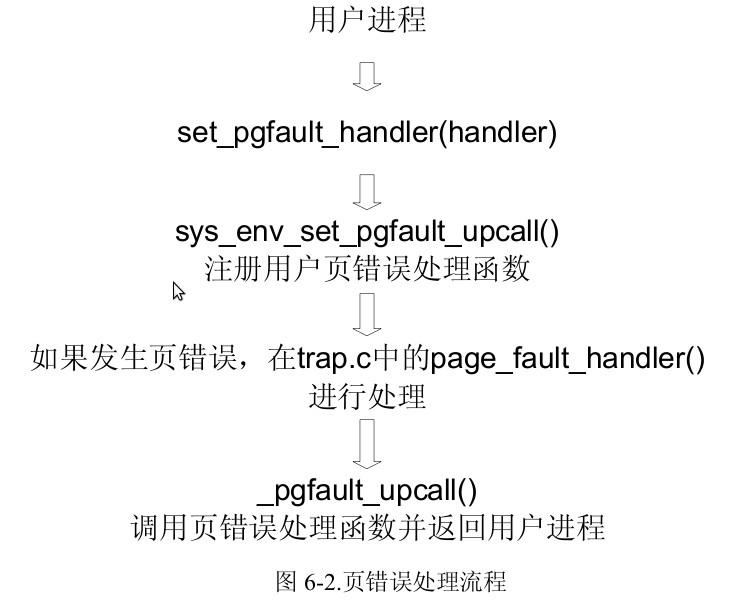
\includegraphics[scale=0.500]{/home/zhangchi/lab/report/pgfault.png}
\end{figure}


然后从上到下梳理一下代码:

\begin{enumerate}
\item{第4行,注意这里调用的是 \funcname{ set\_pgfault\_handler() } 而不是系统调用 \funcname{ sys\_env\_set\_pgfault\_upcall() },\highlight{ 因为前者会检查用户程序的错误栈是否存在 },如果没有则分配相应空间。我们无法得知父进程在调用fork前是否已经为错误栈分配了空间,所以不能直接调用后者}
\item{第22行,拷贝从0到UXSTACKTOP之间的所有用户页面。因为我们在创建用户env时,已经在\funcname{env\_setup\_vm()} 中将UTOP(即UXSTACKTOP)之上的所有页面都映射到和内核一样,但是不要映射错误栈的空间,因为我们马上要给它创建新物理页。}
\item{第33行,为子进程设置页错误处理程序。因为使用\funcname{env\_alloc()}创建的env的处理程序指针都为空,但是这时我们已经明确的为其错误栈分配了物理页面,所以可以直接使用系统调用指定错误处理的入口了,\_pgfault\_upcall为所有用户页错误处理程序的总入口。}

\end{enumerate}

至此使用Copy on Write机制的fork函数就完成了,运行用户程序forktree能争取打印出Exercise要求的结果。任务完成!





\section{Preemptive Multitasking and Inter-Process communication (IPC)}

\subsection{Clock Interrupts and Preemption}

\subsubsection{Interrupt discipline}

\subsubsection{Handling Clock Interrupts}

\subsection{Inter-Process communication (IPC)}

\subsubsection{IPC in JOS}

\subsubsection{Sending and Receiving Messages}

\subsubsection{Transferring Pages}

\subsubsection{Implementing IPC}


\begin{lstlisting}[style=console]
\end{lstlisting}

\begin{lstlisting}[style=console]
\end{lstlisting}



\begin{lstlisting}[style=exercise]
\end{lstlisting}


\begin{lstlisting}[style=exercise]
\end{lstlisting}

\begin{lstlisting}[style=exercise]
\end{lstlisting}


\begin{lstlisting}[style=exercise]
\end{lstlisting}

\begin{lstlisting}[style=acode, title={\scriptsize \ttfamily \bfseries kern/trapentry.S}]
\end{lstlisting}

\begin{lstlisting}[style=acode, title={\scriptsize \ttfamily \bfseries kern/trapentry.S}]
\end{lstlisting}

\begin{lstlisting}[style=acode, title={\scriptsize \ttfamily \bfseries kern/trapentry.S}]
\end{lstlisting}








\begin{lstlisting}[style=console]
\end{lstlisting}

\begin{lstlisting}[style=exercise]
\end{lstlisting}



\begin{lstlisting}[style=acode, title={\scriptsize \ttfamily \bfseries kern/trapentry.S}]
\end{lstlisting}


\clearpage

\end{CJK*}
\end{document}
	

e